\documentclass{article}
\usepackage{amsmath}
\usepackage{amsthm}
\usepackage{amsfonts}
\usepackage{amssymb}
\usepackage{bbold}
\usepackage{dsfont}
\usepackage{graphicx}
\usepackage{cleveref}
\usepackage{bm}
\usepackage{booktabs}
\usepackage{siunitx}
\usepackage{xcolor}
\usepackage[utf8]{inputenc}
\usepackage[english]{babel}
\newtheorem{definition}{Definition}
\newtheorem{example}{Example}
\newcommand{\exP}[1]{\mathrm{e}^{#1}}
\newcommand{\dif}{\mathrm{d}}
\renewcommand{\vec}[1]{\mathbf{#1}}
\newcommand{\pdagger}{{\phantom{\dagger}}}
\newcommand{\state}[1]{\vert #1\rangle}
\newcommand{\cstate}[1]{\langle #1\vert}
\newcommand{\tr}[1]{\mathrm{tr}\left\{#1\right\}}
\newcommand{\trs}[2]{\, \mathrm{tr}_{#1}\{#2\}}
\newcommand{\expc}[3]{\langle #1\vert #2 \vert #3\rangle}
\usepackage[doi=false,url=false,isbn=false,backend=bibtex,style=nature,natbib=true,sorting=none]{biblatex}
\bibliography{bib.bib}
\usepackage{geometry}
\geometry{
	a4paper,
	total={170mm,257mm},
	left=20mm,
	top=20mm,
}
\begin{document}
\title{Report 12: Fixing the units and some questions on the integrator}
\author{Rudolf Smorka}
\maketitle
\section{Units}
The Hamiltonian is of the form
\begin{equation}
	\hat{h} = \sum_{j,k} h_{jk}^\pdagger \hat{c}_j^\dagger \hat{c}_k^\pdagger + \sum_{j,k}\alpha_{jk}^\pdagger (\hat{c}_j^\dagger \hat{c}_k^\pdagger+\mathrm{h.c.}) (\hat{a}_j^\dagger + \hat{a}_j) + \sum_j \hbar \omega_j \left(\hat{a}^\dagger_j \hat{a}^\pdagger_j+\frac{1}{2}\right)
\end{equation}
with the annihilation and creation operators
\begin{equation}
	\hat{a}_j = \sqrt{\frac{m\omega}{2\hbar}} \left(\hat{x}_j + \frac{i}{m_j\omega_j}\hat{p}_j\right), \qquad \hat{a}_j^\dagger = \sqrt{\frac{m_j\omega_j}{2\hbar}} \left(\hat{x}_j - \frac{i}{m_j\omega_j}\hat{p}_j\right).
\end{equation}
Dimensionless coordinates and momenta are defined as
\begin{equation}
	\hat{X}_j = \sqrt{\frac{m_j\omega_j}{\hbar}} \hat{x}_j, \qquad \hat{P}_j = \frac{\hat{p}_j}{\sqrt{\hbar m_j\omega_j}}
\end{equation}
with which the ladder operators can be redefined
\begin{equation}
	\hat{a}_j = \frac{1}{\sqrt{2}}(\hat{X}_j+i\hat{P}_j), \qquad \hat{a}_j^\dagger = \frac{1}{\sqrt{2}}(\hat{X}_j-i\hat{P}_j).
\end{equation}
Within the Ehrenfest approximation, the vibrational operators are replaced with their expectation values, which are assumed to be classical. Within this approximation and assuming that all vibrational modes have the same frequency, the semiclassical Hamiltonian from above becomes
\begin{align}
	h_\mathrm{sc} = \sum_{j,k}h_{jk}^\pdagger \hat{c}_j^\dagger \hat{c}_k^\pdagger + \sum_{j,k}\frac{\alpha_{jk}}{\sqrt{2}} (c_j^\dagger c_k^\pdagger + \mathrm{h.c.})X_j +  \hbar \omega \sum_{j} \frac{1}{2}\left(X_j^2+P_j^2+\frac{1}{2}\right)
\end{align}
The dimensionless semiclassical Hamiltonian is then obtained by dividing the above Hamiltonian by $\hbar \omega$
\begin{align}
	H = \sum_{j,k}H_{jk}^\pdagger c_j^\dagger c_k^\pdagger + \sum_{j,k}\frac{A_{jk}}{\sqrt{2}} (c_j^\dagger c_k^\pdagger + \mathrm{h.c.})X_j +  \sum_{j}\frac{1}{2}\left(X_j^2+P_j^2+\frac{1}{2}\right) = H_\mathrm{el} + H_\mathrm{el-vib} + H_\mathrm{vib}
\end{align}
with $H_{jk} = \frac{h_{jk}}{\hbar\omega}$ and $A_{jk}=\frac{\alpha_{jk}}{\hbar \omega}$.
The Ehrenfest equations of motion for the dimensionless coordinates and momenta under the dimensionless semiclassical Hamiltonian given above are
\begin{align}
	\frac{\dif \rho}{\dif \tau}&= -i[H,\rho] \\
	\frac{\dif X_j}{\dif \tau} &= \frac{\partial \langle H \rangle}{\partial P_j} = P_j\\
	\frac{\dif P_j}{\dif \tau} &= -\frac{\partial \langle H\rangle}{\partial X_j} =-\sum_k\frac{A_{jk}}{\sqrt{2}} \langle c_{j}^\dagger c_{k}^\pdagger + \mathrm{h.c.}\rangle - X_j.
\end{align}
where the dimensionless time $\tau=\omega t$ has been introduced.
The initial coordinates and momenta are sampled from either the Wigner representation of the thermal Gibbs state
\begin{equation}
	\rho_W^\mathrm{G}(X,P) = \prod_j 2\alpha_j \exP{-\alpha_j (X_j^2+P_j^2)}\label{eq:Wigner_Thermal}
\end{equation}
with $\alpha_j = \tanh\left(\frac{\beta\hbar\omega_j}{2}\right)$,
or the Wigner representation of the ground state
\begin{equation}
	\rho_W^\mathrm{GS}(X,P) = \prod_j 2 \exP{-X_j^2-P_j^2}.
\end{equation}
\section{Sampling of initial classical variables}
The classical coordinates and momenta at initial time are sampled from $\rho_W(X,P)$ by using the Box-Muller transform with rescaled transformed variables. For $u_1,u_2\sim \mathcal{U}_{[0,1)}$, the coordinates and momenta are given by
\begin{align*}
	X_0 &= \sqrt{\frac{-2\log (u_1)}{\alpha}} \cos(2\pi u_2),\\
	P_0 &= \sqrt{\frac{-2\log (u_1)}{\alpha}} \sin(2\pi u_2).\\
\end{align*}
In \cref{fig:Wigner_sampling} the result of sampling using the above Box-Muller transform is compared to the analytical Wigner representation $\rho_W^{\mathrm{G}}(X,P)$ of the thermal state $\rho^G$.  \Cref{fig:Wigner_sampling} (a) shows the analytical $\rho_W^\mathrm{G}(X,P)$ and (b) the sampled one in phase space. \Cref{fig:Wigner_sampling} (c) and (d) show cuts along the $P=0$ and $X=0$ axis, respectively, where the histogram shows the sampled data and the feint orange line is the analytical result.
\begin{figure}[!h]
	\centering
	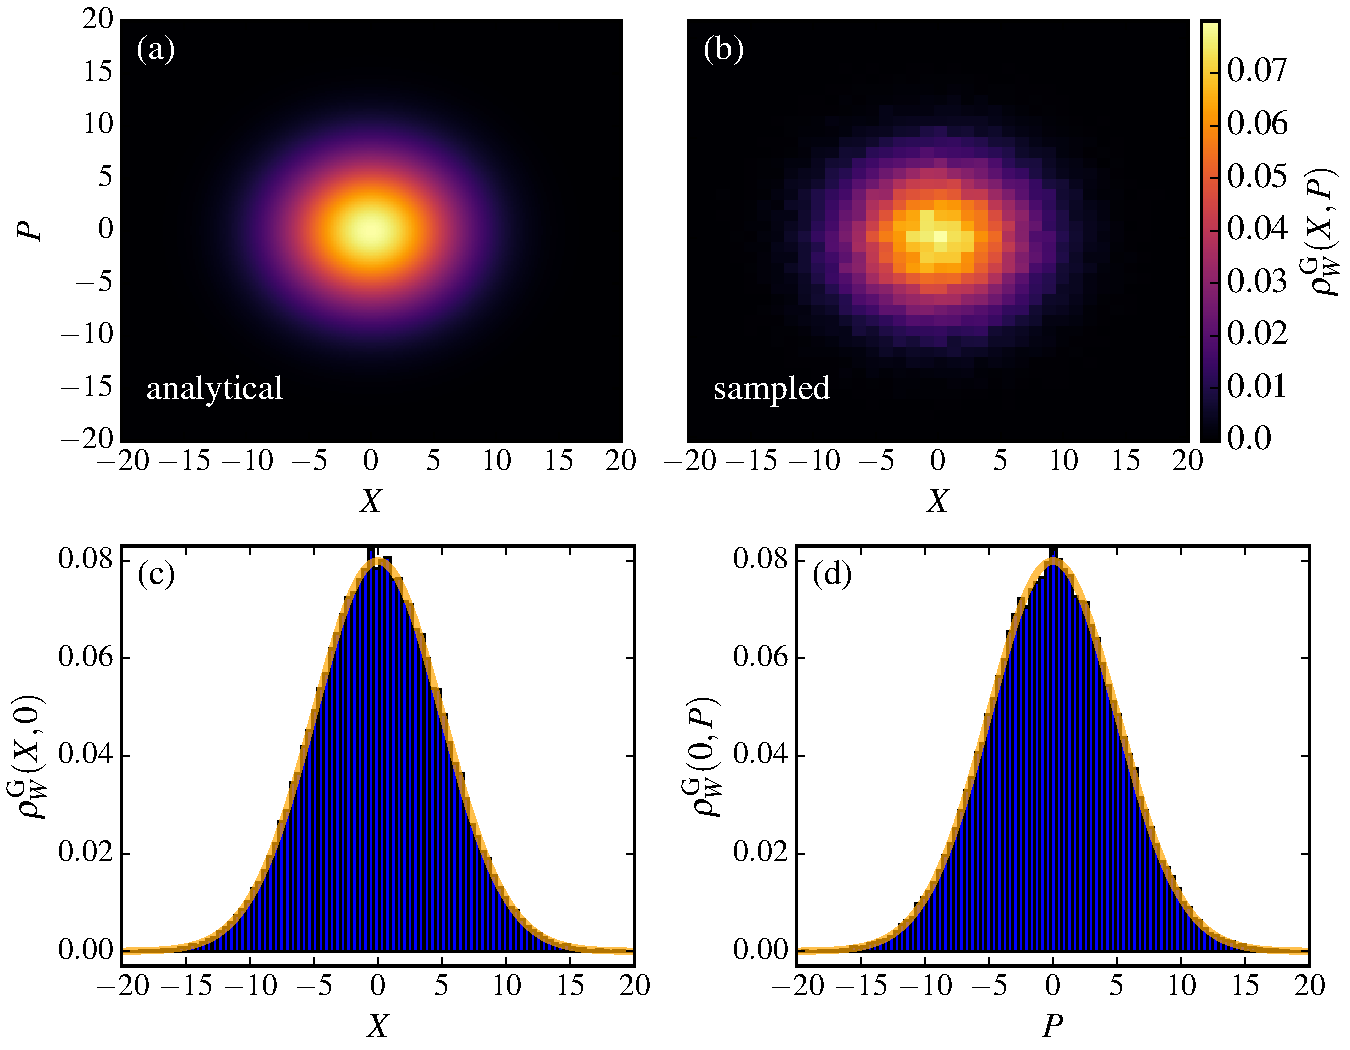
\includegraphics[width=0.9\textwidth]{figs/Comparison_sampled_Wigner.pdf}
	\caption{Comparison between analytical and sampled Wigner distribution $\rho_W^\mathrm{G}(X,P)$ of the thermal state.}\label{fig:Wigner_sampling}
\end{figure}
\section{Time-propagation}
The system of coupled differential equations for the reduced density matrix, the first tier auxiliary density matrices, and the classical canonical variables takes the following form
\begin{align*}
	\frac{\dif}{\dif \tau}\rho &= -i[H_\mathrm{el}+H_\mathrm{el-vib},\rho] + \sum_\ell (\Pi_\ell^\dagger + \Pi_\ell^{\phantom{\dagger}}) \\
	\Pi_\ell(t) &= \frac{1}{4}(\mathds{1}-2\rho)\Gamma_\ell-\sum_{p=1}^{N_p} \Pi_{\ell,p}(t)\\
	\frac{\dif}{\dif t} \Pi_{\ell,p}(t) &= -\frac{i\eta_p}{\beta_\ell}\Gamma_\ell - i\left(H_\mathrm{el}+H_\mathrm{el-ph}-\frac{i}{2}\Gamma-\chi_p^+\mathds{1}\right)\Pi_{\ell,p}(t)\\
	\frac{\dif P_j}{\dif \tau}&= -X_j - \tr{\rho \nabla_{X_j}H_\mathrm{el-vib}}, \\
	\frac{\dif X_j}{\dif \tau} &=  P_j.
\end{align*}
Here, the level-width matrices $\Gamma_\ell$ are dimensionless.
In the previous reports, results where obtained for the following integration strategy:
\begin{itemize}
	\item[i.] Propagate electronic matrices: $\rho(t_n) , \Pi_{\ell,p}(t_n)$ (with $t_n = n\Delta t$) obtained from $\rho(t_{n-1}),\Pi(t_{n-1}), X(t_{n-1}),P(t_{n-1})$ using  Runge-Kutta 4th order with fixed time-step $\Delta t$
	\item[ii.] Propagate classical vectors: $X(t_n),P(t_n)$ obtained from $X(t_{n-1}),P(t_{n-1}),\rho(t_{n-1})$ using symplectic Euler with same $\Delta t$ as in the electronic propagation
\end{itemize}
Alternative integration strategies exist. In the following, the same integration strategy as previously is used. However, different integrators with a fixed step size are explored. For the electronic dynamics, Runge-Kutta 4th order is used and for the vibrational dynamics 
\begin{itemize}
	\item[1.] symplectic Euler (1st order) 
	\item[2.] symplectic Verlet (2nd order) 
	\item[3.] symplectic Ruth (3rd order) \cite{ruth1983canonical}
	\item[4.] symplectic Forest-Ruth (4th order)\cite{forest1990fourth}
	\item[5.] Runge-Kutta 4th order
\end{itemize}
There exist symplectic integrators with adaptive step size. However, it seems to me that additional problems are introduced compared to a fixed step size integrator. For example (as discussed in \cite{richardson2011symplectic}), when the variable step size (generally a function of $X,P,$ and $t$) satisfies $\Delta(X,P,t) \dif t = \dif \tau$, then the classical equations of motion are equivalent to the following equations of motion
\begin{align*}
	\frac{\dif X}{\dif \tau} &= \frac{1}{\Delta(X,P,t)}\frac{\partial H}{\partial P}\\
	\frac{\dif P}{\dif \tau} &= -\frac{1}{\Delta(X,P,t)}\frac{\partial H}{\partial X}\\
	\frac{\dif t}{\dif \tau} &= \frac{1}{\Delta(X,P,t)}
\end{align*}
by simply changing the time variable from $t$ to $\tau$ and integrating above equations with a fixed step size $\Delta \tau = h$. The system of equation above is not a canonical Hamiltonian system. 

For a time-dependent adaptive time step of the form $\Delta(t)=\Delta_0 (1+\varepsilon\cos(\Omega t))$ (using a symplectic Leapfrog integrator), the authors of \cite{richardson2011symplectic} have shown that instabilities arise in the one-dimensional harmonic oscillator ($H=\frac{\omega}{2}(Q^2+P^2)$) if 
\begin{equation*}
	\left\vert\omega-\frac{\Omega}{2}\right\vert < \frac{\omega^2 \Delta_0\varepsilon}{4}.
\end{equation*}
Therefore, we will test integrators with a fixed step size only.

In an isolated system ($\Gamma_\ell = 0$), dynamics is unitary in the quantum subsystem, and symplectic in the classical subsystem. It can be shown, that the quantum-classical equations of motion have a symplectic structure, by decomposing the wavefunction coefficients $c_j = \frac{1}{\sqrt{2}}(q_j+ip_j)$ and solving the equation of motion for $c_j$ from the time-dependent Schrödinger equation.
Additionally to conserved quantities due to symmetries of the Hamiltonian, the trace of the density matrix is constant $\mathrm{tr}\{\rho\}=N$ and the total energy 
\begin{equation*}
	E(t) = \tr{\rho(t)(H_\mathrm{el}+H_\mathrm{el-vib}(t))} + \sum_j \frac{1}{2}\left(X_j^2(t) + P_j^2(t) + \frac{1}{2}\right)
\end{equation*}
is conserved. 
Related to the total energy of the isolated system, one observes that the following equality holds
\begin{align*}
	\dot{W}_\mathrm{el-vib} + \dot{E}_\mathrm{vib} &= 0,\\
	\dot{W}_\mathrm{el-vib} &= \tr{\rho_\mathrm{sys}\dot{H}_\mathrm{el-vib}},\\
	\dot{E}_\mathrm{vib} &= \sum_{j}X_j\dot{X}_j+P_j\dot{P}_j.
\end{align*} 
This is due to the linear electron-vibrational coupling, together with the Ehrenfest approximation, in which one has
\begin{align*}
	\dot{H}_\mathrm{el-vib} &= \sum_{j,k}\frac{A_{j,k}}{\sqrt{2}}\dot{X}_j \\
	&= \sum_{j,k}\frac{A_{j,k}}{\sqrt{2}}P_j \\
	&= \sum_{j} P_j \partial_{X_j}H_\mathrm{el-vib}
\end{align*}
and the change in vibrational energy is 
\begin{align*}
	\dot{E}_\mathrm{vib} &= \sum_{j}X_j\dot{X}_j+P_j\dot{P}_j\\
	&= \sum_{j}(X_jP_j - P_jX_j - P_j\tr{\rho_\mathrm{sys}\partial_{X_j}H_\mathrm{el-vib}})\\
	&= -\tr{\rho_\mathrm{sys}\sum_j P_j \partial_{X_j}H_\mathrm{el-vib}}.
\end{align*}
To find out which combination of integrators yields optimal results, we consider a bond-Peierls model within the Ehrenfest approximation, described by the Hamiltonian
\begin{equation*}
	H =  \sum_{j\sigma}\left(-T_0 + \frac{T_1}{\sqrt{2}}X \right)(c_{j\sigma}^\dagger c_{j\sigma}^\pdagger + \mathrm{h.c.}) 
\end{equation*}
with the vibrational frequency $\hbar \omega = \SI{2}{\milli\electronvolt}$, hopping integral $t_0 = \SI{40}{\milli\electronvolt}$ and Peierls coupling $t_1=\SI{4}{\milli\electronvolt}$ (note that $T_0=t_0/(\hbar \omega)$ and $T_1=t_1/(\hbar\omega)$, as defined above in the dimensionless Hamiltonian). The initial position and momenta of the two bond-modes are
\begin{equation*}
	(X_0^{(1)},P_0^{(1)}) = (1,0.4), \qquad (X_0^{(2)},P_0^{(2)}) = (-1,-2)
\end{equation*} 
and the electronic system is initialized in an empty chain with an electron on the first site with spin up
\begin{equation*}
	\rho_0 = \begin{pmatrix}
		1 &0& \dots& 0\\
		0 &0& \dots& 0\\
		\vdots &\ddots&\dots& \vdots \\
		0 & \dots & \dots & 0
	\end{pmatrix},
\end{equation*}
which is far away from the ground state and therefore dynamics is oscillatory.
\Cref{fig:L3_Iso_tot_Energy} (a) shows the time-evolution of the absolute deviation of the total energy from the initial total energy. The different lines show results obtained with different integrators for the classical equation of motion. In all cases, a Runge-Kutta 4th order integrator has been used for solving the electronic equation of motion.
Note the logarithmic scale and the offset by $10^{-9}$ to show results which are numerically zero. The time-step in the electronic in vibrational integrators are set to $dt=0.0001$ (in dimensionless units; in dimensioned units, $dt=\SI{0.012}{\femto\second}$), except for the symplectic Euler integrator, where two different time steps have been used for comparison of the error. 
\Cref{fig:L3_Iso_tot_Energy} (b) shows the trace of the density matrix, and \cref{fig:L3_Iso_tot_Energy} (c) the quantity $\dot{W}_\mathrm{el-vib}+\dot{E}_\mathrm{vib}$.
\begin{figure}[!h]
	\centering
	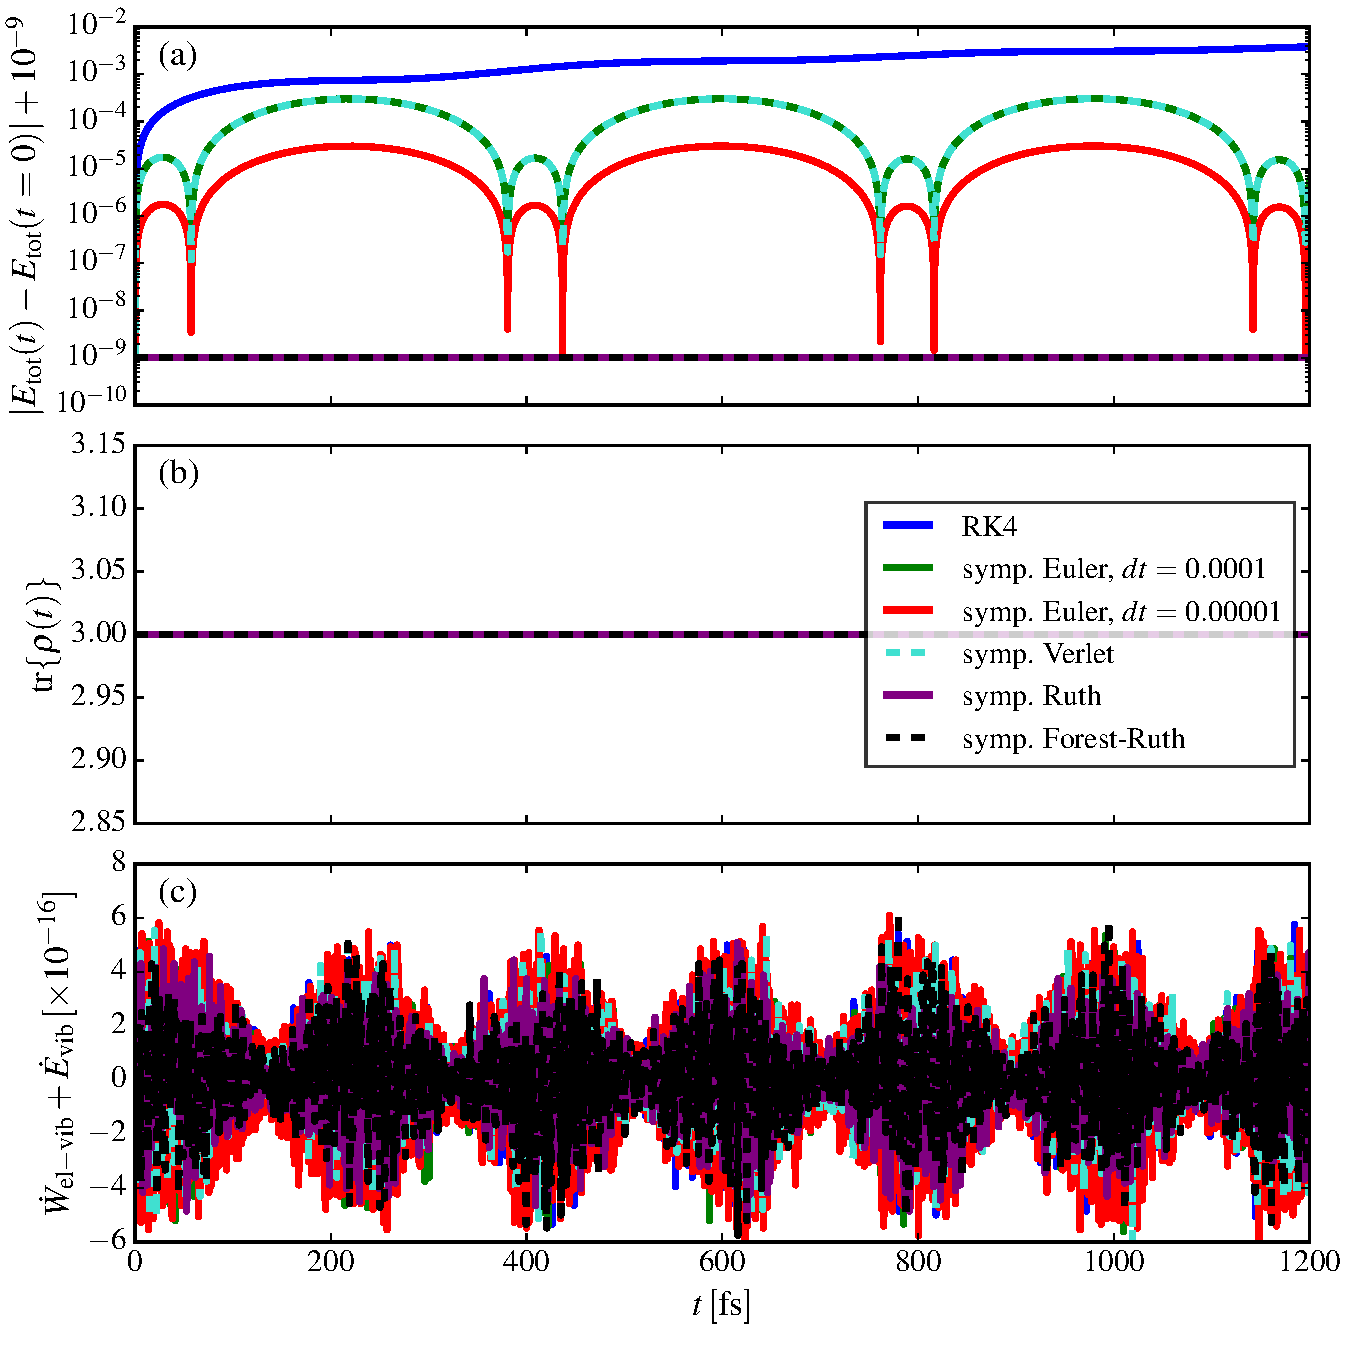
\includegraphics[width=1.0\textwidth]{figs/L3_coupled_iso_integrators.pdf}
	\caption{Comparison of integration errors for different integrators in the isolated Bond-Peierls model.}\label{fig:L3_Iso_tot_Energy}
\end{figure}
\newpage
Figure commentary:
\begin{itemize}
	\item Integration error is clearly visible in the total energy. The other quantities are conserved for all integrators and thus do not provide a measure of the error as useful as the total energy.
	\item Using a non-symplectic integrator (in this case, RK4, blue line) for the classical equation of motion leads to an error which is orders of magnitude larger than using a symplectic integrator with a lower convergence order (e.g. symplectic Euler, green line). The error also increases with time in this case.
	\item Symplectic integrators with convergence order 1 or 2 (green, red and turquoise lines) lead to periodically oscillating error, which does not grow in time as fast as the error acquired using the non-symplectic integrator
	\item Only symplectic integrators with convergence order 3 and 4 lead to an error-free (in the sense of errors below machine precision) integration (purple and black lines)
	\item Conclusion: Use at least Ruth (3rd order) symplectic integrator to obtain optimal results. Performance-wise all investigated symplectic integrators lead to approximately the same runtime. This is because the numerically heavy part is integrating the electronic equations of motion.
\end{itemize}	
For the case that $\Gamma_\ell\neq 0$, the total energy
\begin{equation*}
	E(t) = \tr{\rho_\mathrm{tot}(t)(H_\mathrm{el,sys}+H_\mathrm{el-vib,sys}(t)+H_\mathrm{leads})} + \sum_j \frac{1}{2}\left(X_j^2(t) + P_j^2(t) + \frac{1}{2}\right)
\end{equation*}
is conserved. However, within the used formulation this quantity is not accessible, since $\rho_\mathrm{tot}$ and the leads Hamiltonian $H_\mathrm{leads}$ are not accessible. However, the relation
\begin{equation*}
	\dot{W}_\mathrm{el-vib} + \dot{E}_\mathrm{vib} = 0
\end{equation*}
with $\dot{W}_\mathrm{el-vib}$ and $\dot{E}_\mathrm{vib}$ as defined above holds also for the open system. 
Another thing to check is if for vanishing electron-vibrational coupling, the current-voltage characteristics agrees with the one obtained from Landauer-Büttiker approach, shown in \cref{fig:L3_open_uncoupled} (a) for the model above with $T_1=0$. \Cref{fig:L3_open_uncoupled} (b) shows the deviation of the trace of the reduced density matrix in the steady state from the number of sites and (c) the reduced system energy.
\begin{figure}[!h]
	\centering
	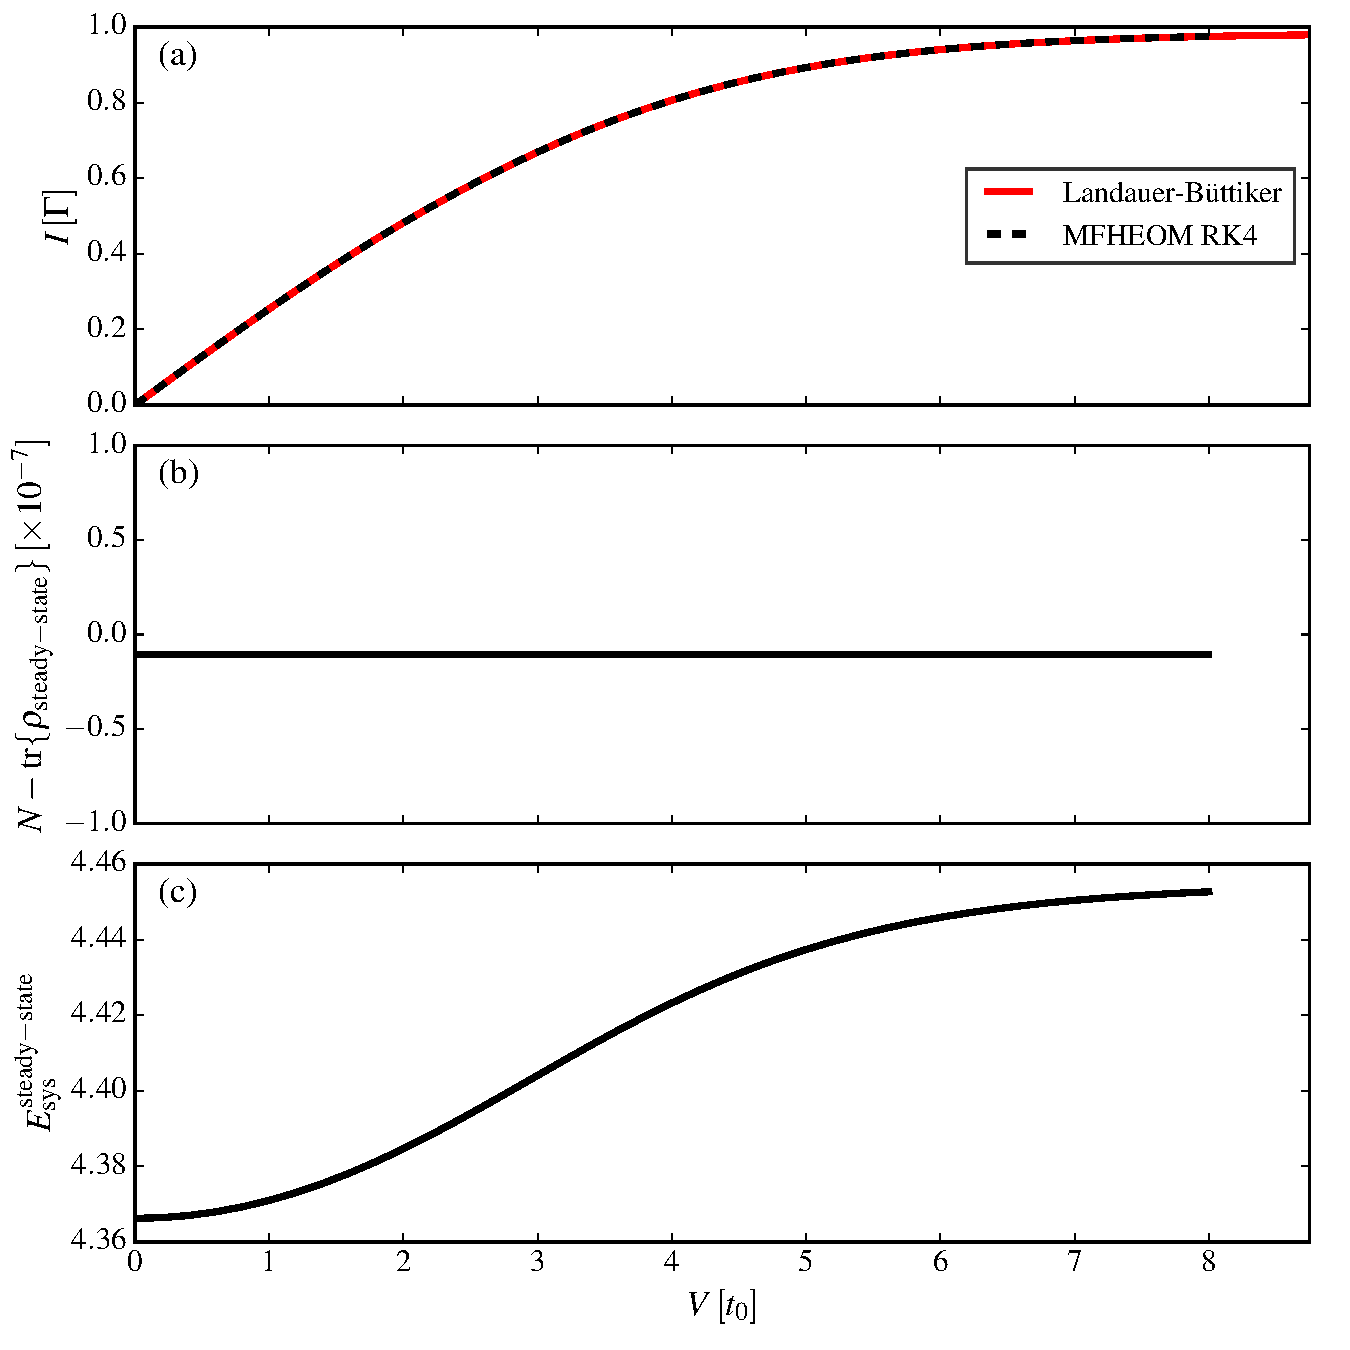
\includegraphics[width=1.0\textwidth]{figs/L3_uncoupled_open.pdf}
	\caption{(a) current-voltage characteristics for a purely electronic problem, (b) deviation of trace of steady-state density matrix from number of sites, (c) steady-state system energy.}\label{fig:L3_open_uncoupled}
\end{figure}
\clearpage
Figure commentary:
\begin{itemize}
	\item The current-voltage characteristics obtained from solving the coupled equations of motion discuseed above agrees perfectly with the one obtained from the Landauer-Büttiker approach.
	\item The trace of the density matrix does not change with voltage (as it should be), and the deviation from the number of sites (the normalization of the single-particle density matrix) is due to the "true" steady-state is reached after longer time than the one which was used for the propagation. A longer time has to be used to make this quantity go to zero.  
	\item  The system energy changes with voltage, which one can explain with states above Fermi-level which get populated in the steady state. 
\end{itemize}
\section{Convergence of time propagation with step size}
We consider the Fransson model 
\begin{align*}
	H&=\sum_{j,\sigma} E_{j\sigma}^\pdagger \hat{c}_{j\sigma}^\dagger \hat{c}_{j\sigma}^\pdagger + \sum_{j\sigma} \left(-T_0 + \frac{T_1}{\sqrt{2}}X_j\right)(\hat{c}_{j\sigma}^\dagger \hat{c}_{j+1,\sigma}^\pdagger + \mathrm{h.c.}) +\\& \sum_{j\sigma\sigma'}\left(\lambda_0 + \frac{\lambda_1}{\sqrt{2}}X_j \right) (i\hat{c}_{j\sigma}^\dagger (\vec{v}_j^{(+)}\cdot \bm{\sigma})_{\sigma\sigma'}^\pdagger \hat{c}_{j+2,\sigma'}^\pdagger + \mathrm{h.c.}) + \sum_j \frac{1}{2}\left(X_j^2 + P_j^2+\frac{1}{2}\right)
\end{align*}
coupled to two leads at the terminating sites. The following parameters
\begin{align*}
	\hbar \omega &= \SI{2}{\milli\electronvolt}\\
	t_0 &= \SI{40}{\milli\electronvolt}\\
	\varepsilon &= -6t_0\\
	t_1 &= 0.1t_0\\
	\lambda_0 &= \frac{t_0}{40}\\
	\lambda_1 &= 0.1\lambda_0\\
	\Gamma_0 &= \frac{t_0}{4}\\
	T &= \SI{25}{\milli\electronvolt}\\
	V &=4t_0.
\end{align*}
The initial density matrix is obtained using the partition-free approach, in which the electronic system is 
in equilibrium with the leads. The initial coordinates and momenta are drawn from the Wigner representation of the thermal state of a harmonic oscillator, \cref{eq:Wigner_Thermal}. A single trajectory calculation is made for varying time step size to check the convergence of the time propagation.






\printbibliography

\end{document}

